\documentclass[../AnalysisNoteJBuxton.tex]{subfiles}


\begin{document}

\subsubsection{Results: \LamKs and \LamKpm: Fit Method Comparisons}
\label{ResultsLamK_FitMethComp}

In Figure \ref{fig:FitResults_ShareR_Sharelam_PolyBgd}, we show extracted fit parameters for the case of \LamKchPALamKchM sharing radii with \LamKchMALamKchP.  The figure shows results for three different treatments of the non-femtoscopic background: a polynomial fit to THERMINATOR 2 simulation to model the background (circles), a linear fit to the data to model the background (squares), and the Stavinsky method (crosses).


\begin{figure}[h]
  \centering
  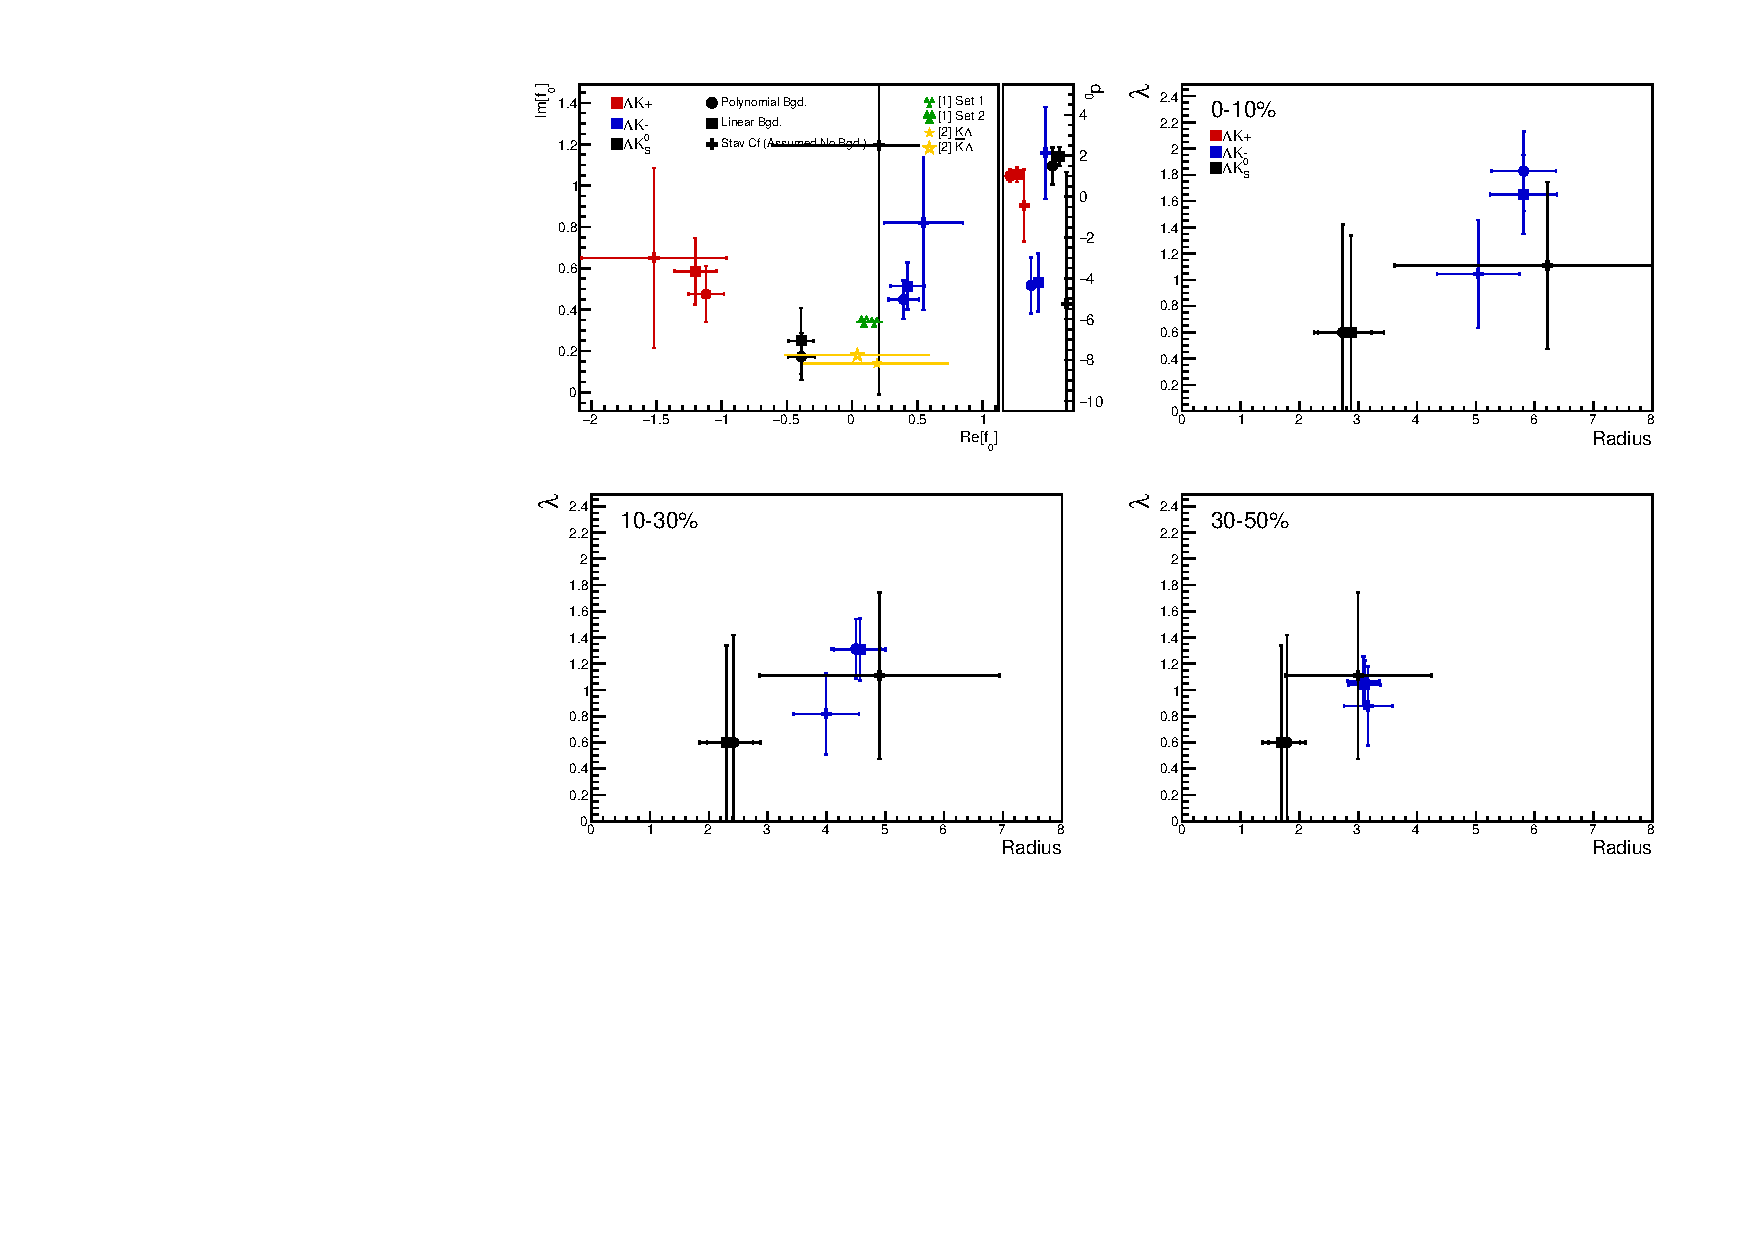
\includegraphics[width=\textwidth]{7_ResultsAndDiscussion/Figures/CompareAllScattParams_CompBgdTreatment_StatOnly.pdf}
  \caption[Compare Fit Parameters: Background treatment]{Compare Fit Parameters: Background treatment: Extracted fit results for all of our \LamALamKpm systems across all studied centrality bins (0-10\%, 10-30\%, 30-50\%).  The \LamKchPALamKchM and \LamKchMALamKchP systems share both a radius and a $\lambda$ parameter for each centrality bin (i.e. 3 total radius parameters, 3 total $\lambda$ parameters).  The figure shows results for three different treatments of the non-femtoscopic background: a polynomial fit to THERMINATOR 2 simulation to model the background (circles), a linear fit to the data to model the background (squares), and the Stavinsky method (crosses).  The green \cite{Liu:2006xja} and yellow \cite{Mai:2009ce} points show theoretical predictions made using chiral perturbation theory.}
  \label{fig:FitResults_ShareR_Sharelam_PolyBgd}
\end{figure}


\begin{figure}[h]
  \centering
  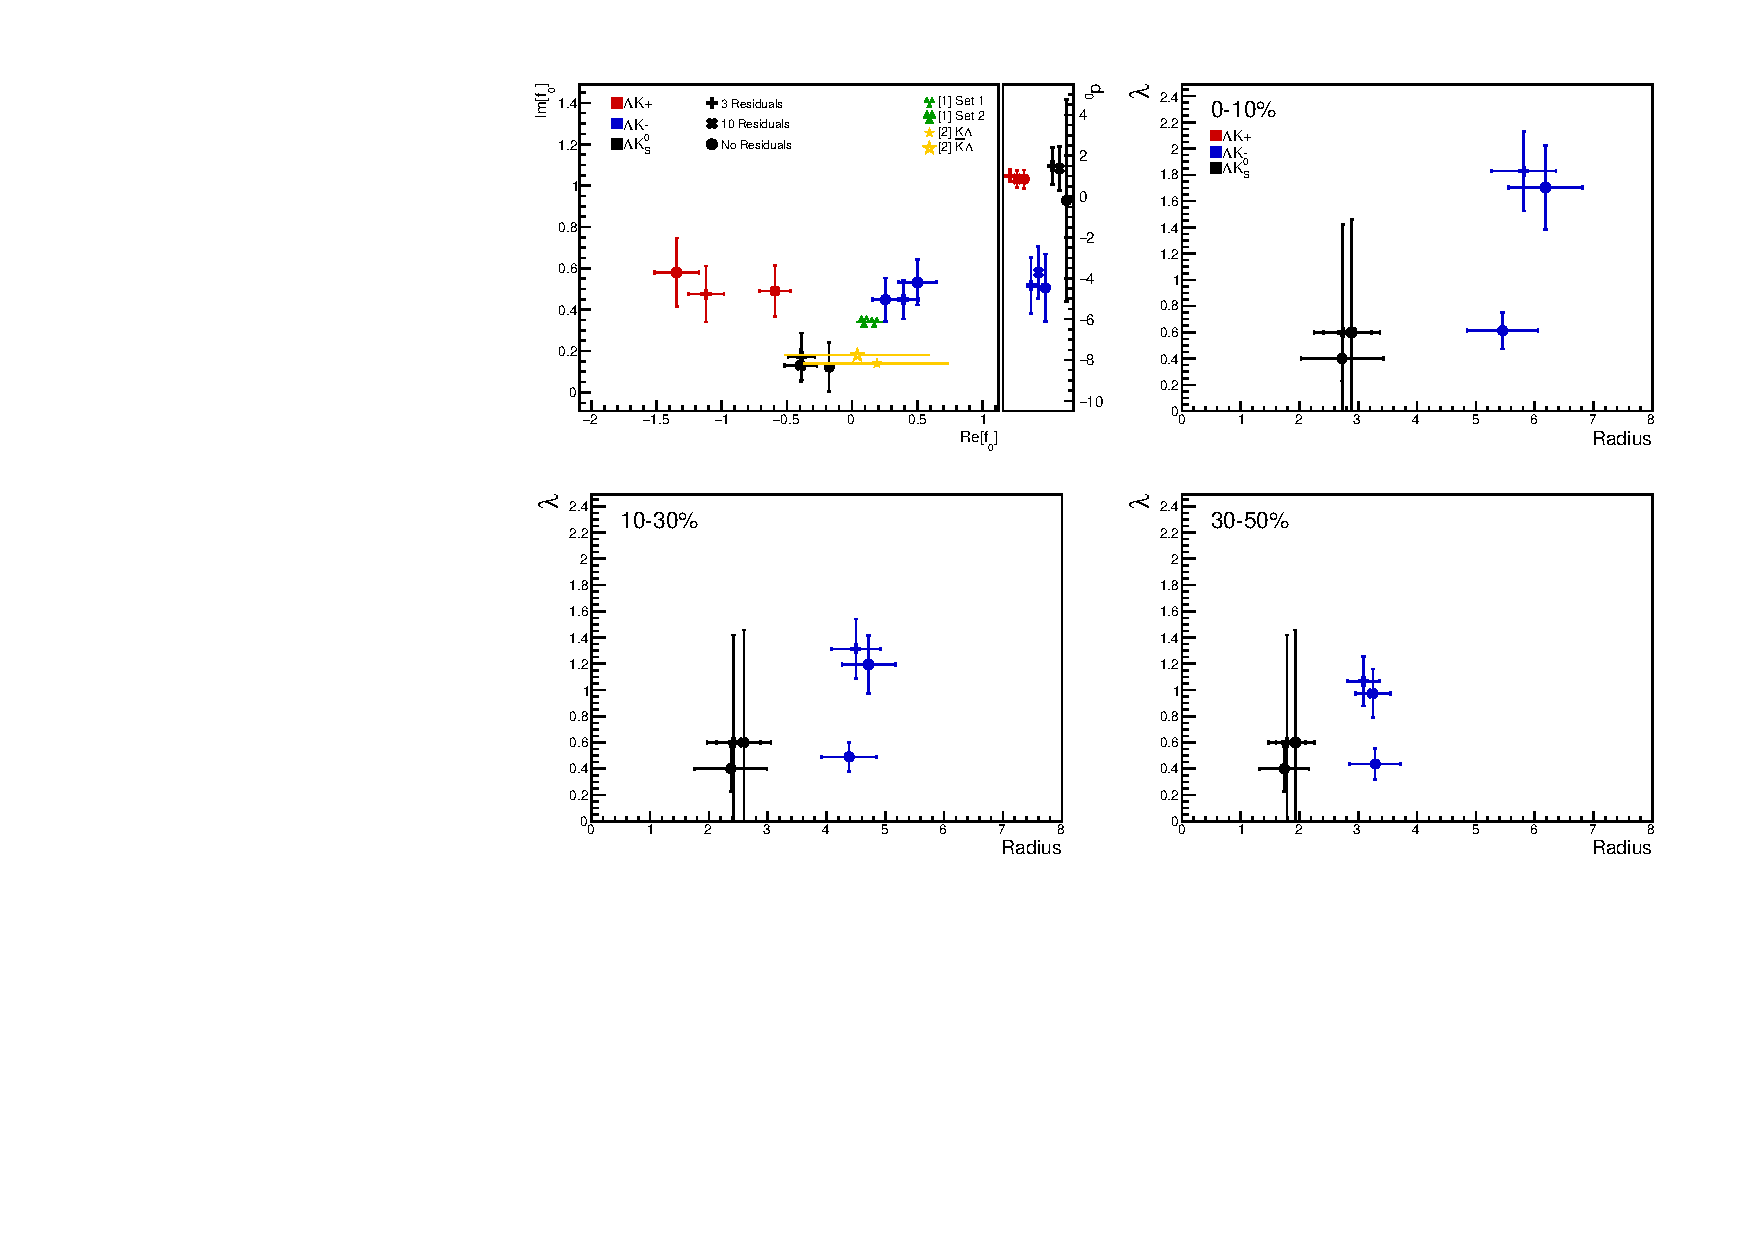
\includegraphics[width=\textwidth]{7_ResultsAndDiscussion/Figures/CompareAllScattParams_CompNumRes_StatOnly.pdf}
  \caption[Compare Fit Parameters: Number of residuals]{Compare Fit Parameters: Number of residuals: Results shown for the case of 3 (+), 10 (X), and no (circles) residual contributors.}
  \label{fig:CompareAllScattParams_CompNumRes}
\end{figure}


\begin{figure}[h!]
  \centering
  %%----start of first subfigure---  
  \subfloat[Shared radii]{
    \label{fig:CompareAllScattParams_FreevsFixlam:a}
    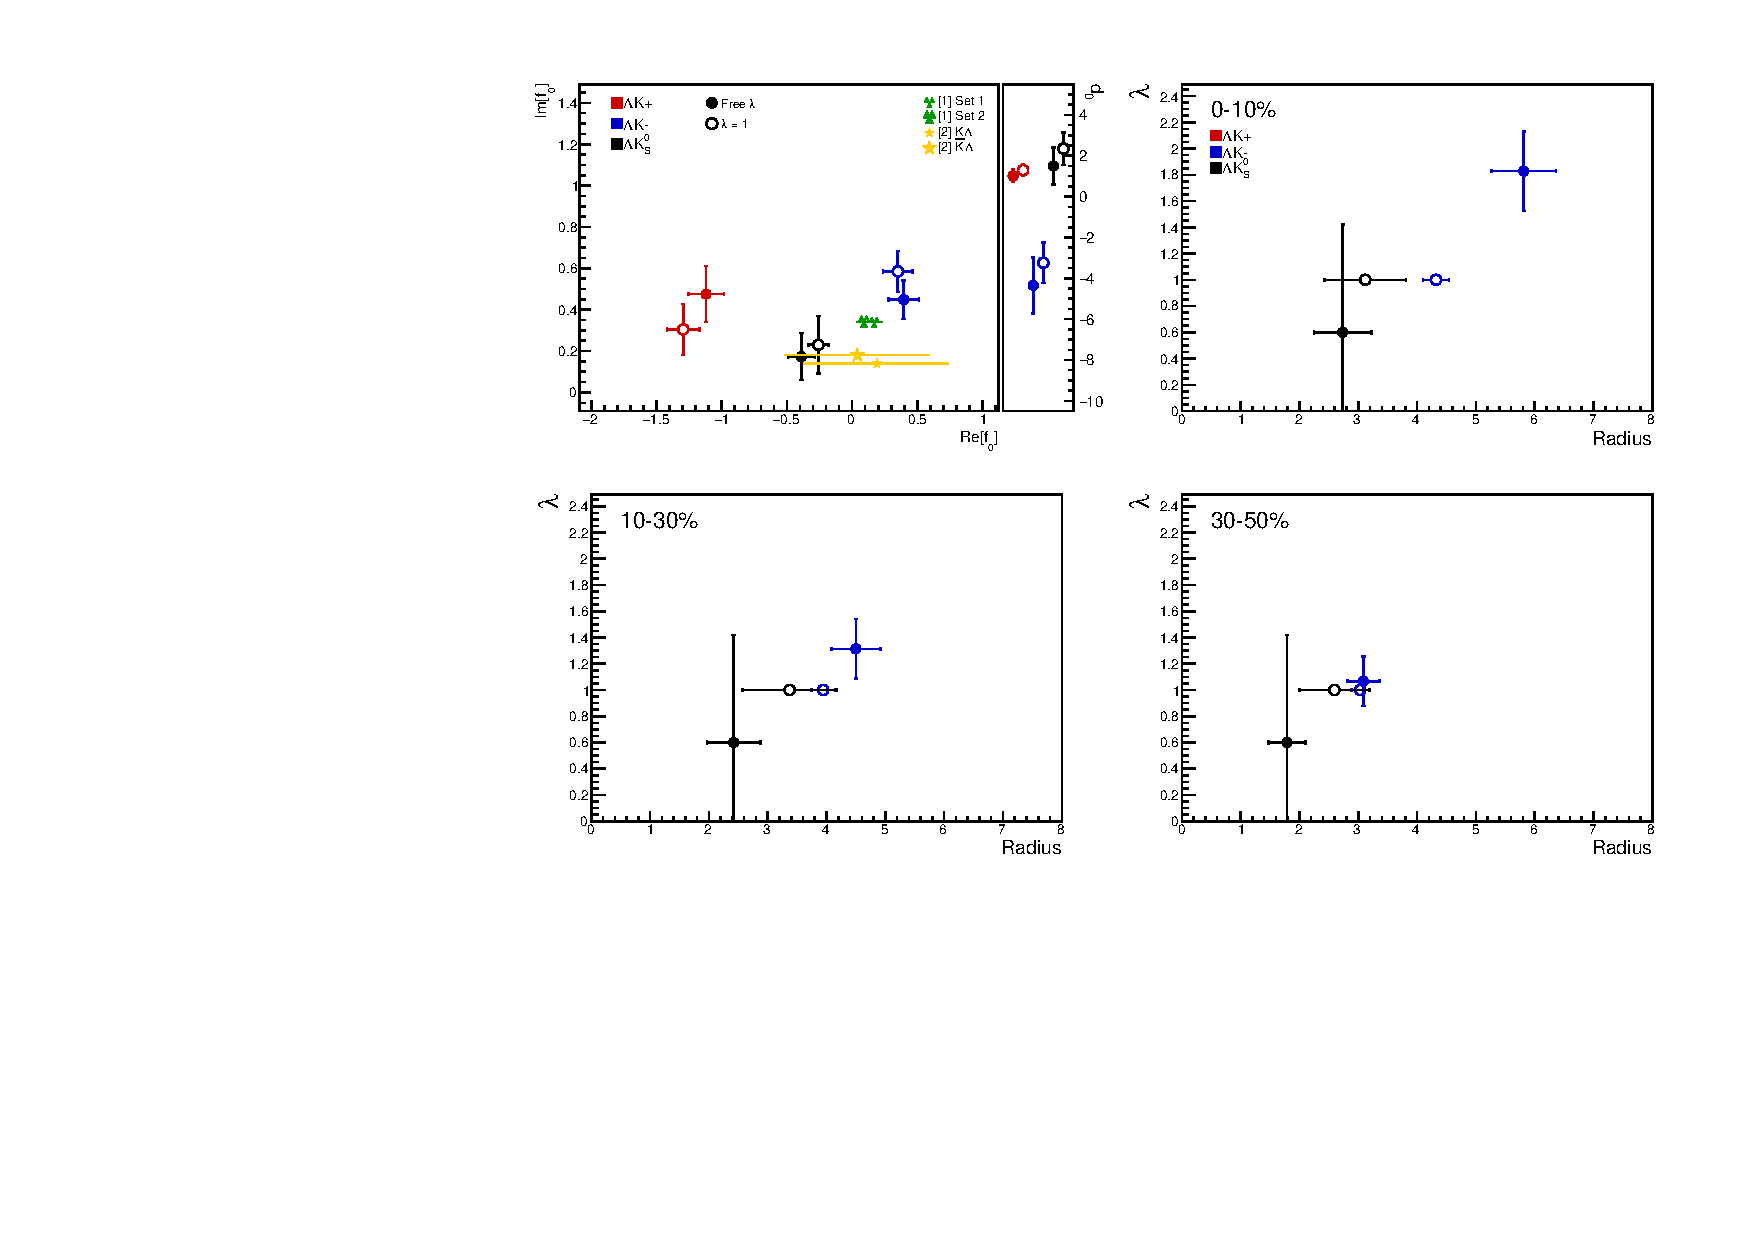
\includegraphics[width=0.750\linewidth]{7_ResultsAndDiscussion/Figures/CompareAllScattParams_CompFreevsFixedlam_ShareR_StatOnly.pdf}}
  \\  
  %%----start of second subfigure---
  \subfloat[Separate radii]{
    \label{fig:CompareAllScattParams_FreevsFixlam:b}
    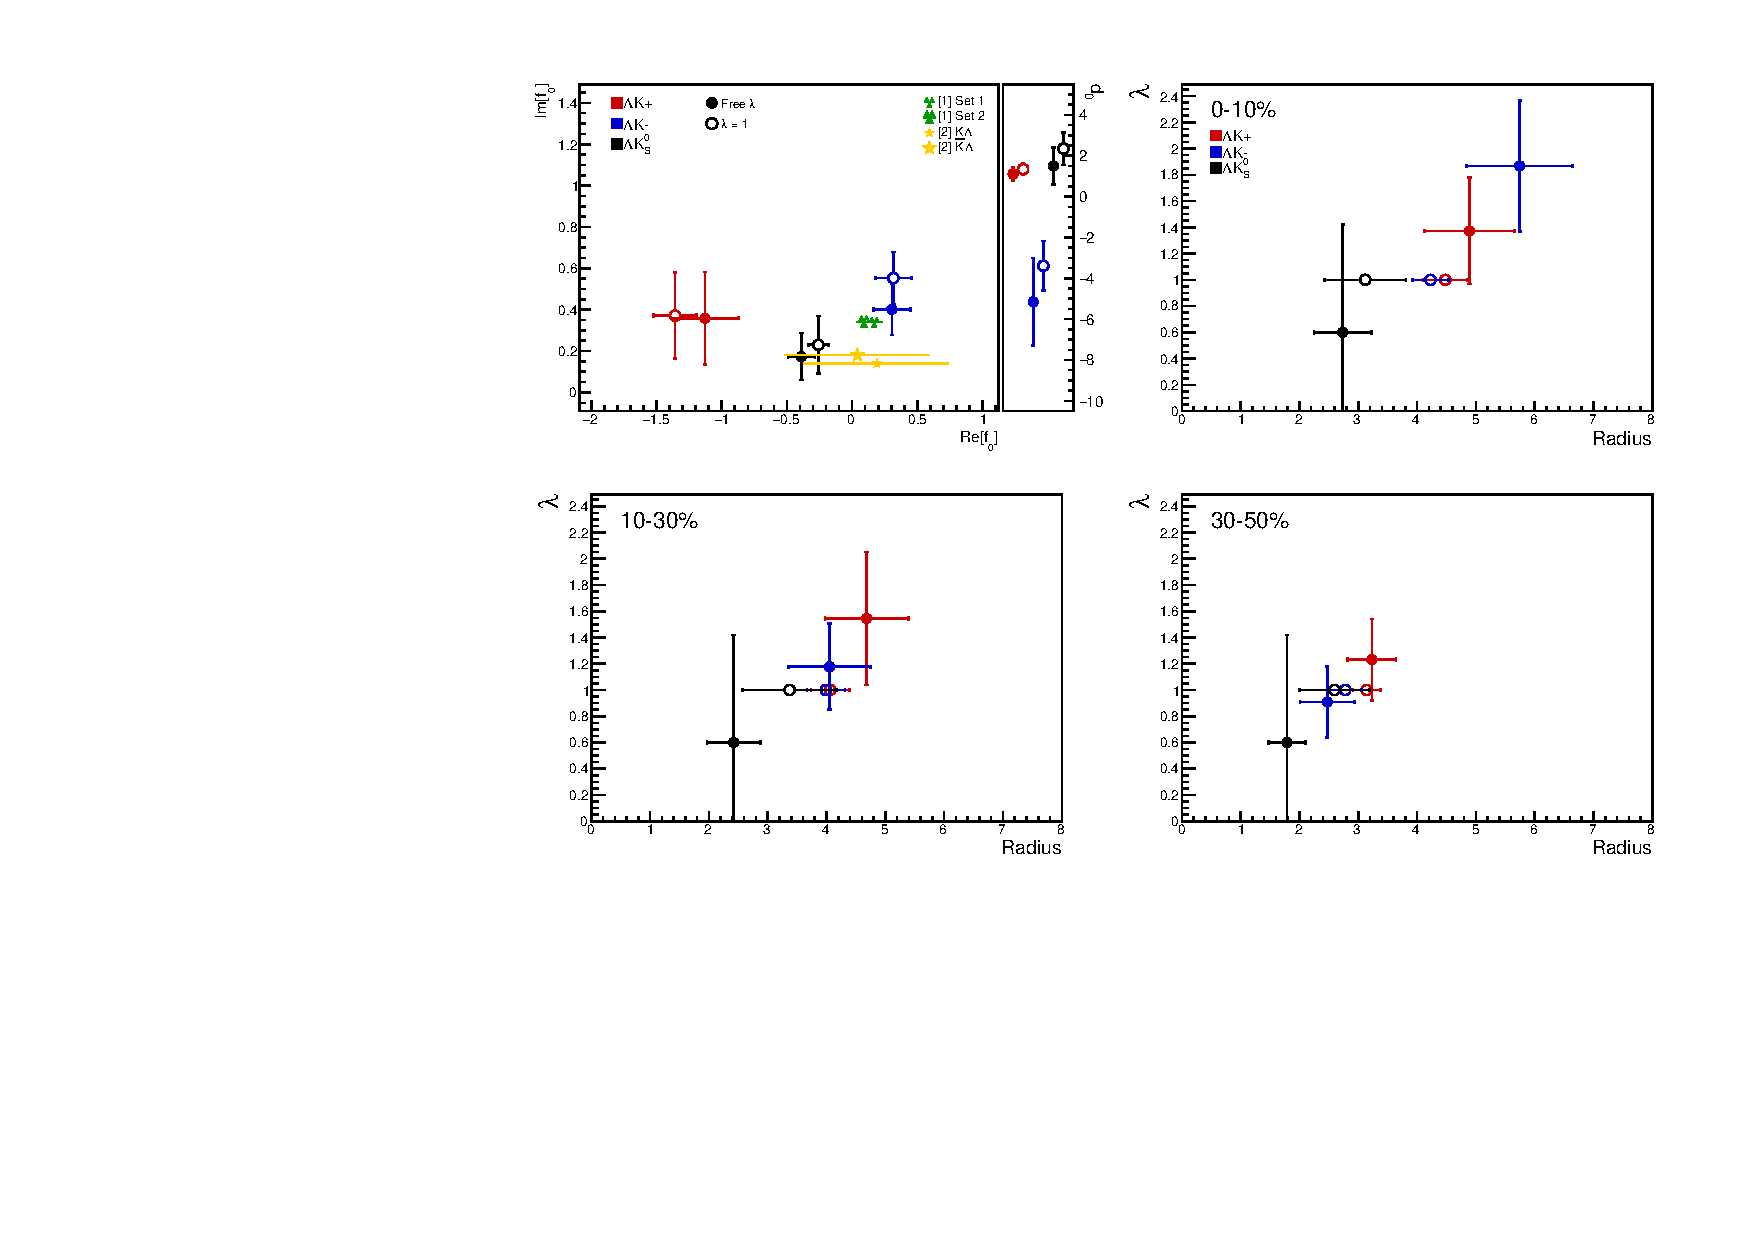
\includegraphics[width=0.750\linewidth]{7_ResultsAndDiscussion/Figures/CompareAllScattParams_CompFreevsFixedlam_SepR_StatOnly.pdf}}  
  %%----overall caption----
  \caption[Compare Fit Parameters: Free vs fixed $\lambda$]{Compare Fit Parameters: Free vs fixed $\lambda$:  Results shown for $\lambda$ parameters left free (filled symbols) and fixed to 1 (open symbols).  In the top plot (\ref{fig:CompareAllScattParams_FreevsFixlam:a}), the \LamKchP and \LamKchM analyses share radii, whereas in the bottom (\ref{fig:CompareAllScattParams_FreevsFixlam:b}) they have unique radii.}
  \label{fig:CompareAllScattParams_FreevsFixlam}
\end{figure}


\begin{figure}[h!]
  \centering
  %%----start of first subfigure---  
  \subfloat[Shared radii]{
    \label{fig:CompareAllScattParams_SharedvsUniquelam:a}
    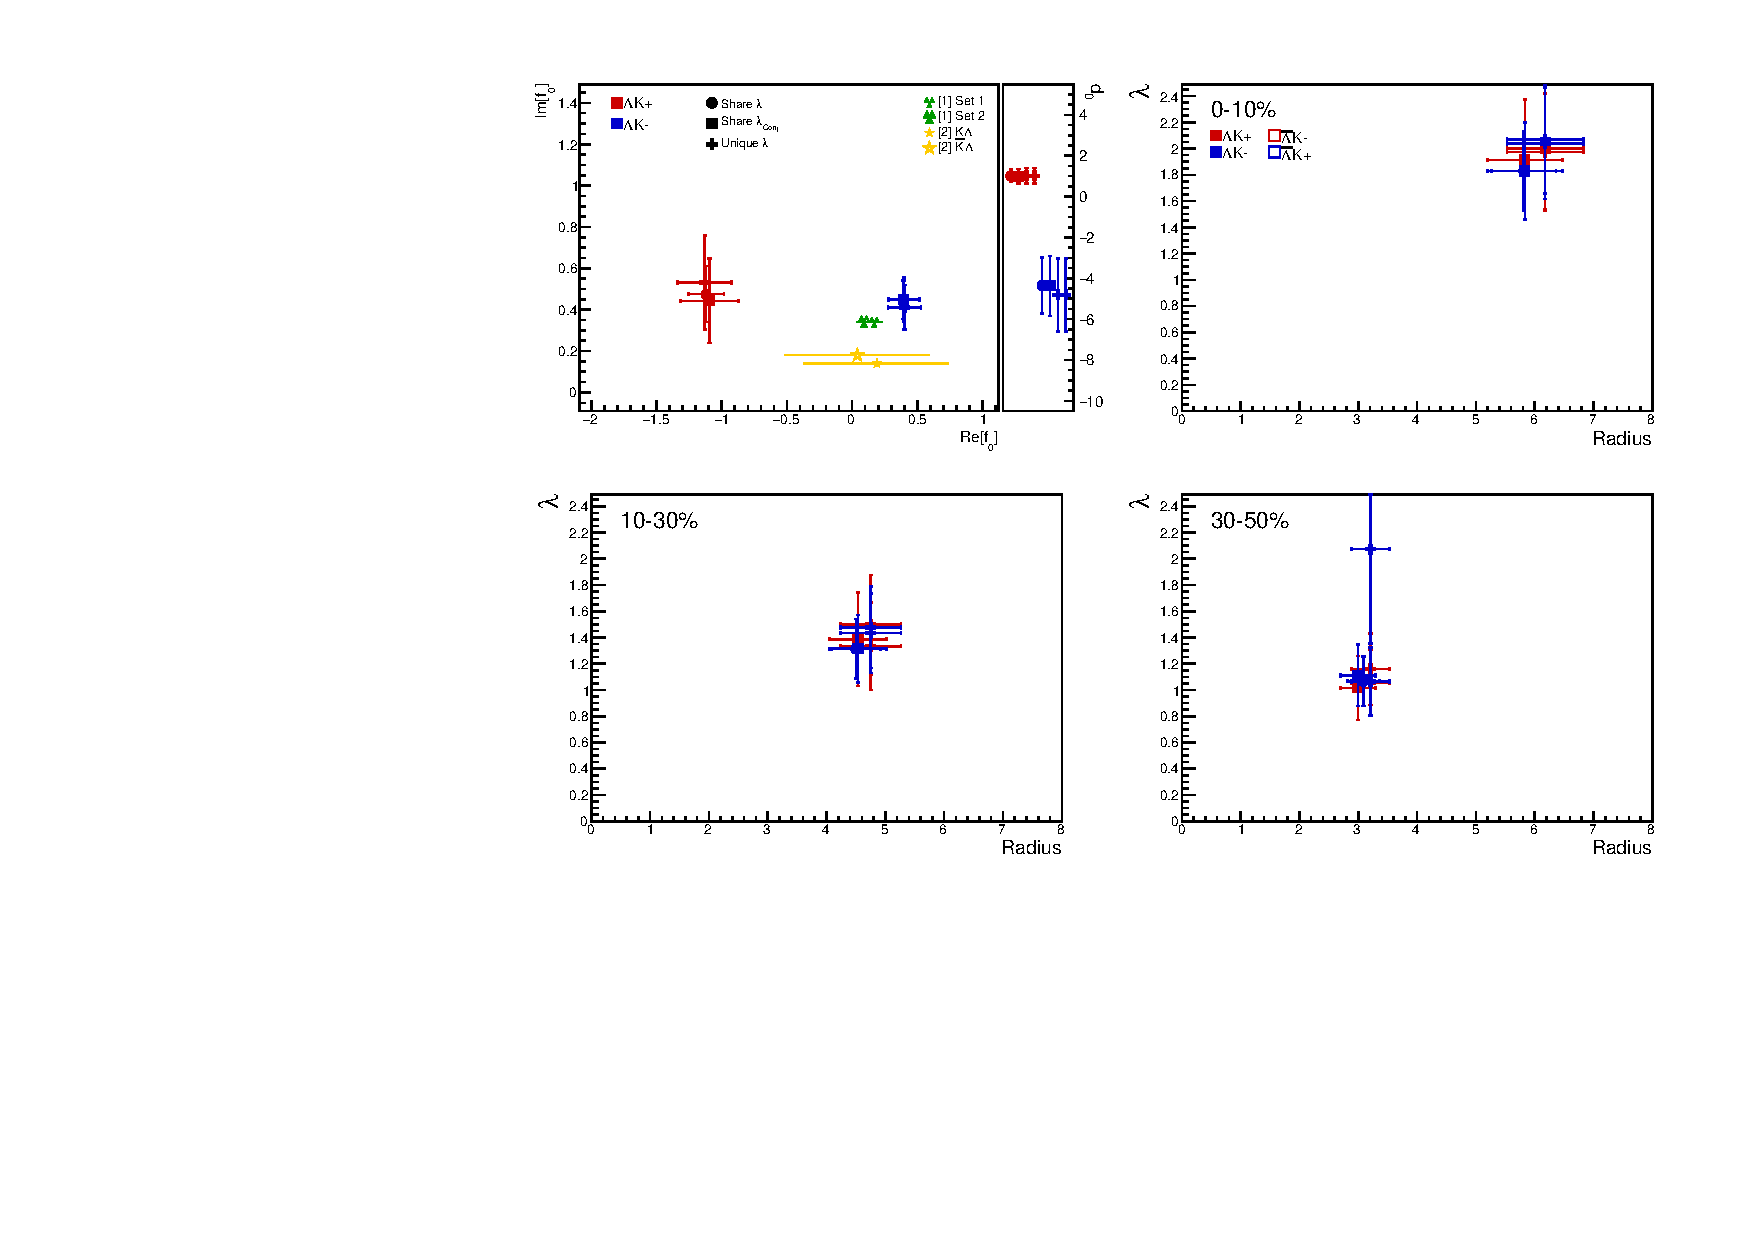
\includegraphics[width=0.750\linewidth]{7_ResultsAndDiscussion/Figures/CompareAllScattParams_CompSharelam_SharedR_StatOnly.pdf}}
  \\  
  %%----start of second subfigure---
  \subfloat[Separate radii]{
    \label{fig:CompareAllScattParams_SharedvsUniquelam:b}
    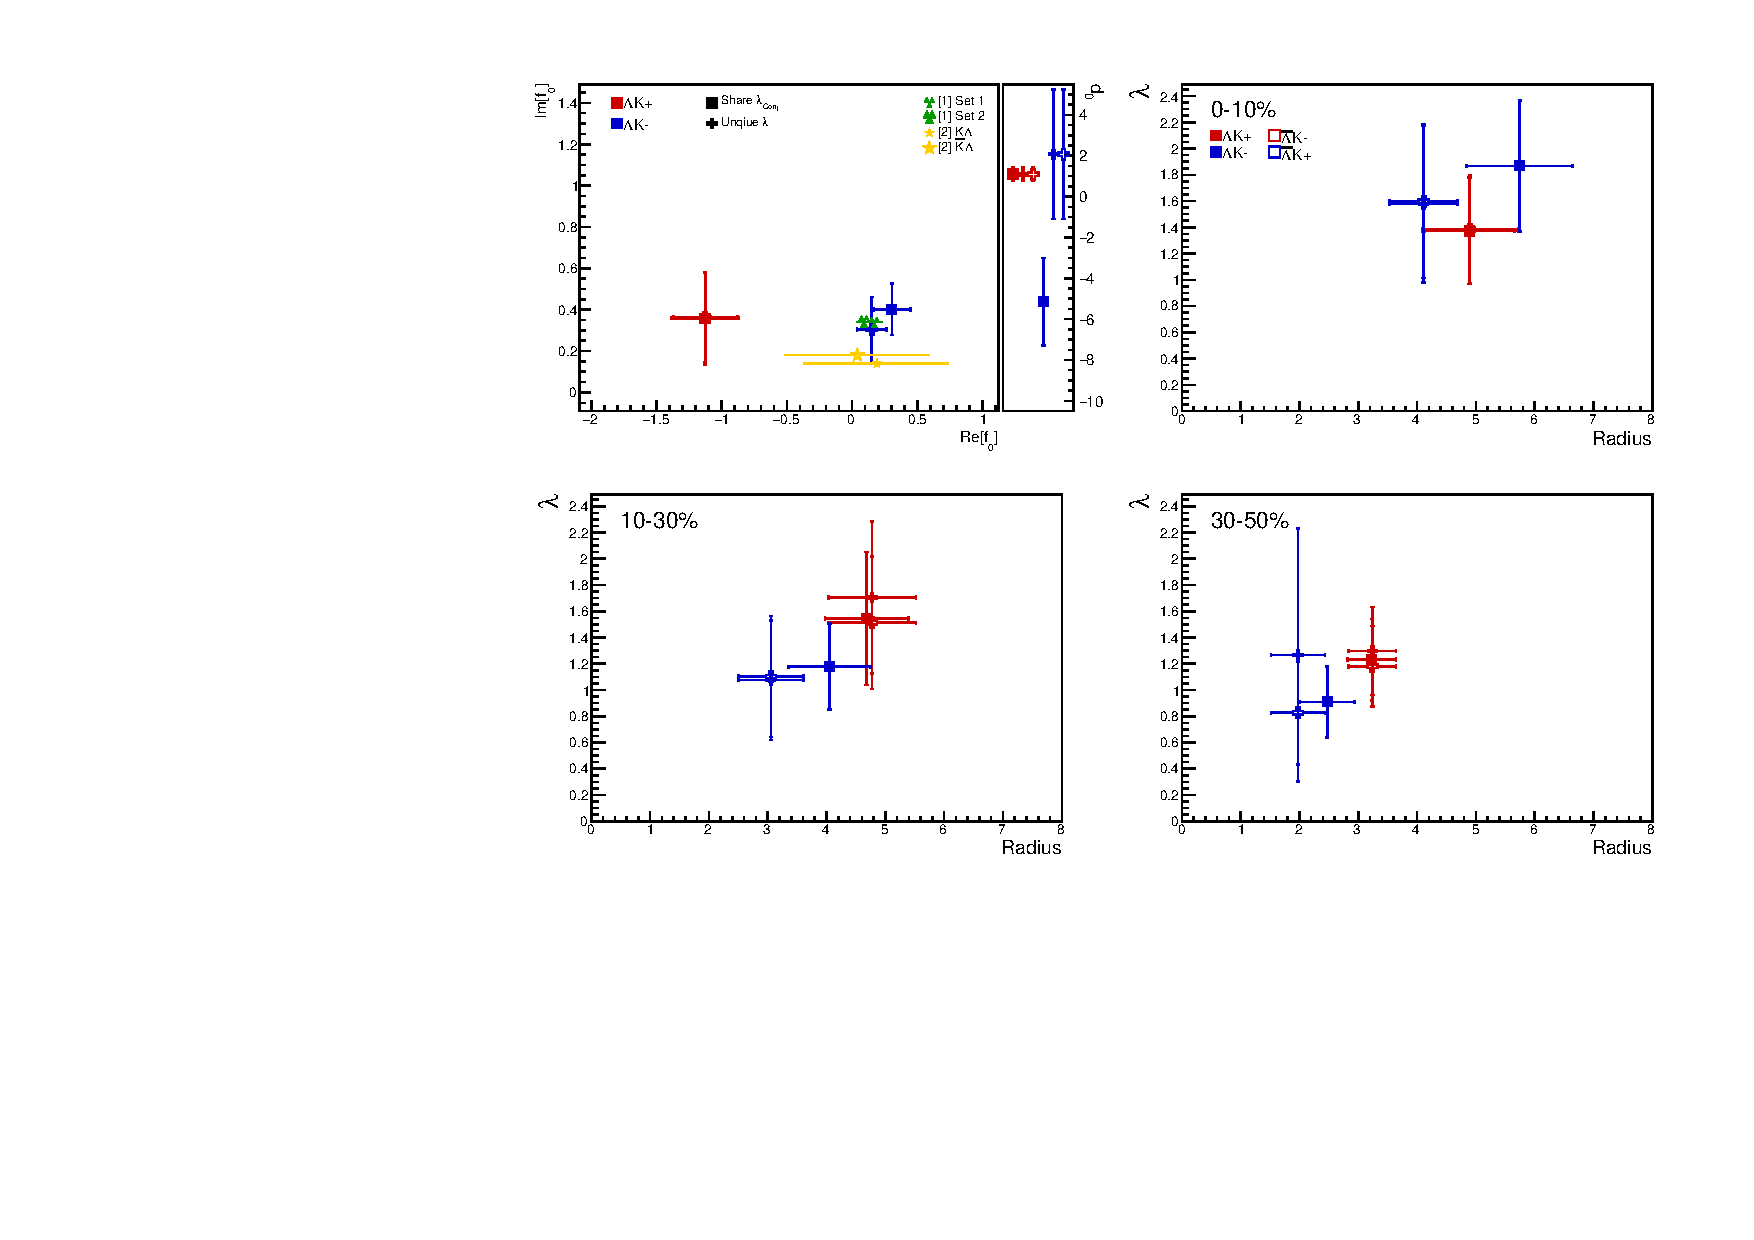
\includegraphics[width=0.750\linewidth]{7_ResultsAndDiscussion/Figures/CompareAllScattParams_CompSharelam_SepR_StatOnly.pdf}}  
  %%----overall caption----
  \caption[Compare Fit Parameters: Shared vs unique $\lambda$]{Compare Fit Parameters: Shared vs unique $\lambda$:  Results shown for different sharing of the $\lambda$ parameters between analyses and systems.  In the top (\ref{fig:CompareAllScattParams_SharedvsUniquelam:a}), the \LamKchP and \LamKchM analyses share radii, whereas in the bottom (\ref{fig:CompareAllScattParams_SharedvsUniquelam:b}), they do not.  ``Share $\lambda$'' (circles) is the case where a single $\lambda$ is shared amongst all analyses for a given centrality bin (i.e., in \ref{fig:CompareAllScattParams_SharedvsUniquelam:a}, 3 radius parameters and 3 $\lambda$ parameters).  ``Share $\lambda_{Conj}$'' (squares) means that conjugate pairs (ex. \LamKchP and \ALamKchM) share a $\lambda$ parameter for each centrality.  This corresponds to 6 total $\lambda$ parameters (for each of the 3 centrality bins, the \LamKchPALamKchM receives a unique $\lambda$, as does \LamKchMALamKchP).  Finally, in ``Unique $\lambda$'' (+), each analysis received its own unique $\lambda$ parameter.  This corresponds to 12 $\lambda$ parameters (for each of the 3 centrality bins, each \LamKchP, \ALamKchM, \LamKchM, and \ALamKchP receives a unique $\lambda$).}
  \label{fig:CompareAllScattParams_SharedvsUniquelam}
\end{figure}



\begin{figure}[h]
  \centering
  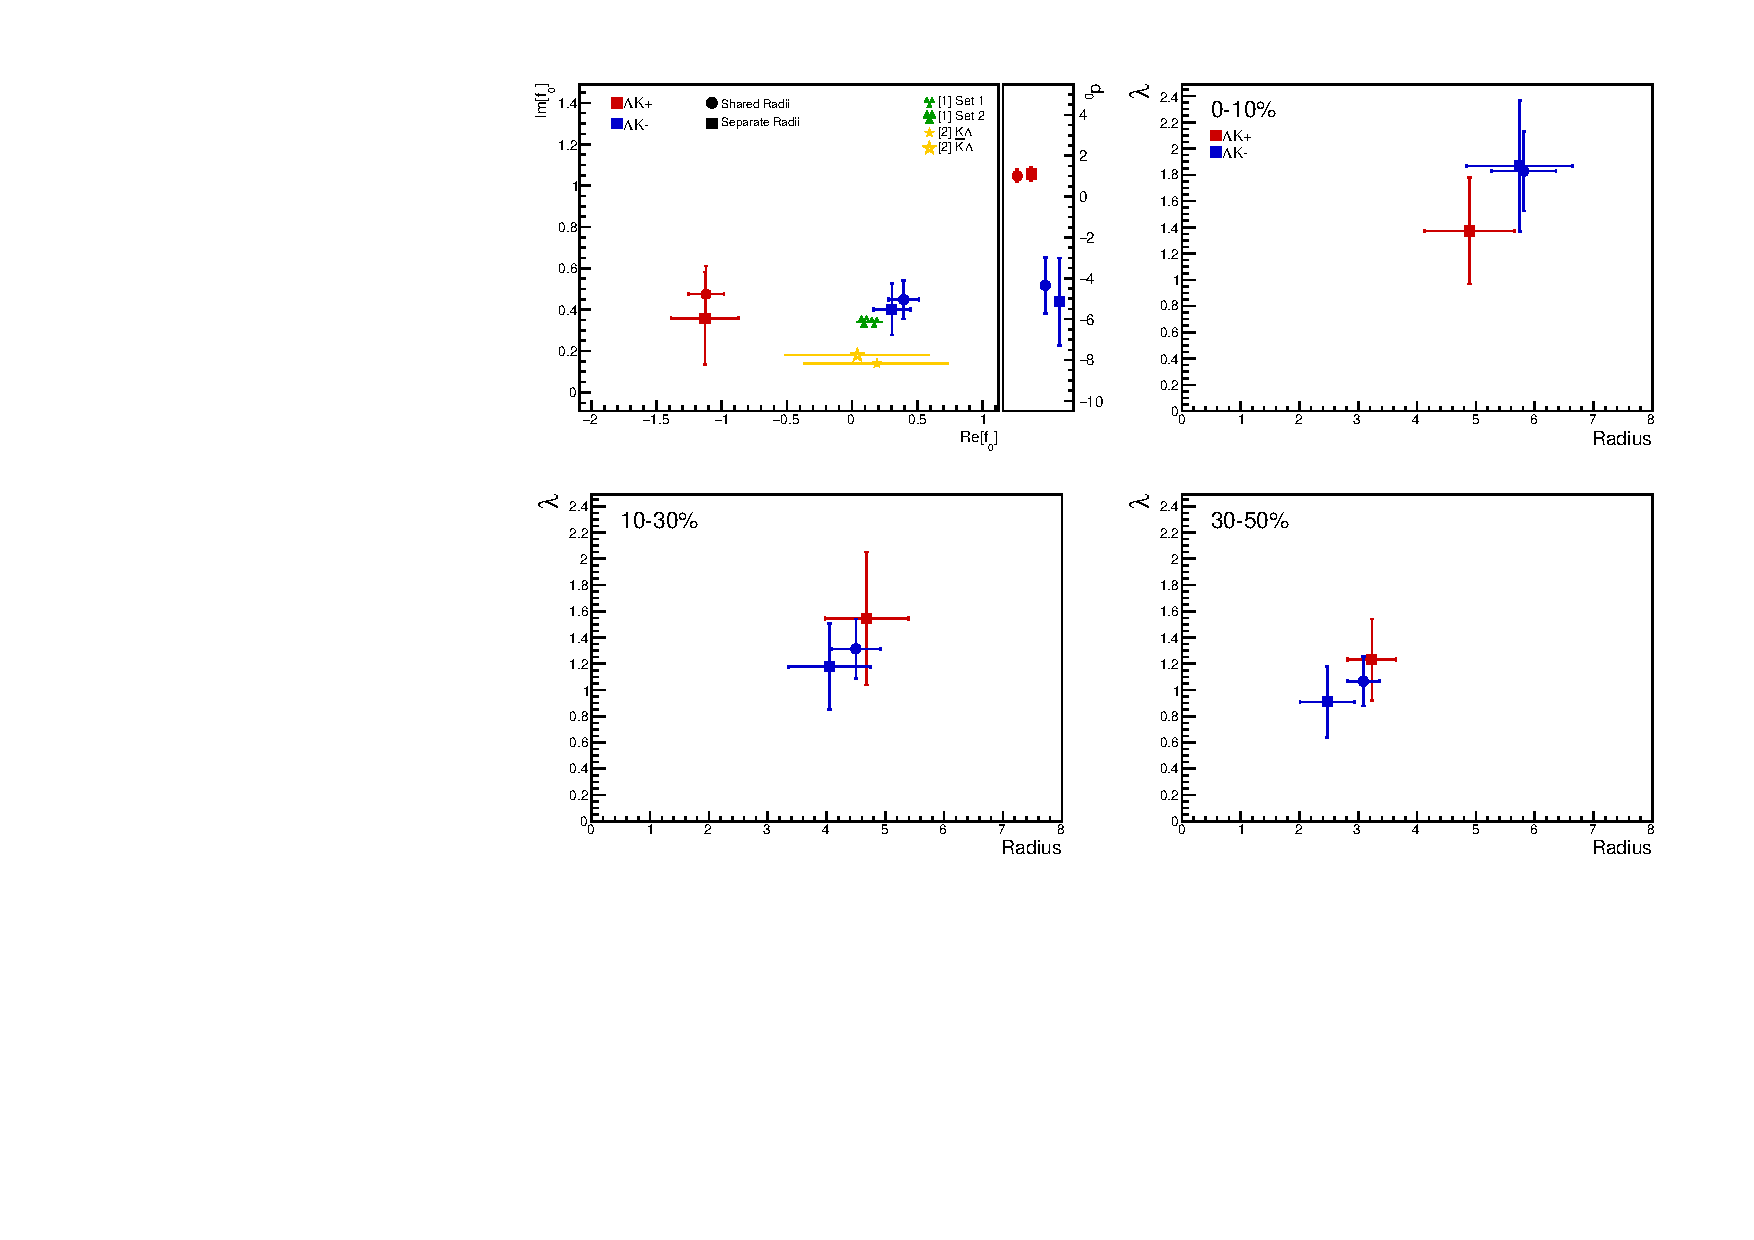
\includegraphics[width=\textwidth]{7_ResultsAndDiscussion/Figures/CompareAllScattParams_CompSharedvsSepR_StatOnly.pdf}
  \caption[Compare Fit Parameters: Shared vs. Separate Radii]{Compare Fit Parameters: Shared vs. Separate Radii:  Results shown for the case of radii being shared between \LamKchPALamKchM and \LamKchMALamKchP (circles) vs not shared (squares).}
  \label{fig:CompareAllScattParams_SharevsSepR}
\end{figure}



\clearpage
\end{document}